\section{Evaluation}\label{sec:evaluation}

The evaluation asks five questions.

\begin{description}[leftmargin=2.6em, style=nextline, itemsep=1pt]
\item[RQ1] Is a certified bound ever exceeded?
\item[RQ2] Does the content rule accept only workflows whose observers cannot tell
  secrets apart, and are its rejections real? How do the two withdrawn rules and the
  classical quantitative bound fare on the same workflows?
\item[RQ3] Are the leakage bounds respected, and how tight are they?
\item[RQ4] What do real tokenizers and a real model say about the assumptions?
\item[RQ5] What happens on real workflows?
\end{description}

\subsection{Setup}\label{sec:eval-setup}

Every number in this section is printed by \code{python bench/evaluate.py}, which exits
with a nonzero status if any assertion fails; \cref{tab:experiments} lists its
experiments. We ran it on a Linux machine with four cores of an Intel Xeon processor
at 2.80\,GHz and 15\,GB of memory, with \code{orchc} built by GCC 13.3, Python 3.11,
tiktoken 0.14.0, Hugging Face \code{tokenizers} 0.20.3 and \code{transformers}
4.46.3~\cite{wolf2020transformers}, and Coq 8.18.0. Every tokenizer, the model and
every source of the real-workflow corpus is pinned to a revision. The plots are drawn by
pgfplots directly from the JSON files that the harness writes, through the script
\file{submission/scp/figures/data.py}, which was written, like the rest of the artifact,
with the help of Claude (Anthropic).

\begin{table}[t]
\centering
\caption{The experiments of \file{bench/evaluate.py}. Each fails the run on any violation.}
\label{tab:experiments}
\small
\begin{tabularx}{\textwidth}{@{}l>{\raggedright\arraybackslash}Xl@{}}
\toprule
& What is checked & RQ \\
\midrule
E0 & counterexamples of both audits are still caught & RQ1, RQ2 \\
E1--E3 & certified bound against 4,600 executions of 23 generated workflows; two simpler bounds for comparison & RQ1 \\
E4 & guaranteed input bound against the content-sensitive tokenizer on byte-bounded variants & RQ1 \\
E5 & three relational rules on 25 workflows, against the observer, under every mode & RQ2 \\
E6 & requests of the size rule's leaking acceptances re-billed with real tokenizers & RQ2 \\
E7 & leakage bounds: certified classes against distinct observations; the interval bound & RQ3 \\
E8 & flow policy on 26 paired secure/insecure workflows & RQ1 \\
E9 & facts about fourteen real tokenizers (\cref{sec:what-fails}) & RQ4 \\
E10 & a real model: output length against request content & RQ4 \\
E11 & 30 real workflows: labels, bounds, re-billing, AgentDojo cross-check & RQ5 \\
\bottomrule
\end{tabularx}
\end{table}

\subsection{RQ1: certified bounds}\label{sec:eval-bounds}

On 23 generated workflows (chains, branches, retries, nesting and wide inputs), 4,600
executions under the estimate model never exceeded the certified total, the output
component or the estimated input component, each checked separately (E1). A flat
per-call sum, which ignores that a retry multiplies its body, was exceeded on 14.9\%
of executions, and a rule that follows control flow but charges a retry body once on
15.4\% (E2). The median slack of the certified bound over the largest observed cost was
1.17, with a range from 1.03 to 1.67 (E3).

The estimate model is the compiler's own, so E4 tests the guaranteed input bound
against something the compiler does not model. On byte-bounded variants of the same
23 workflows, under the content-sensitive tokenizer and both provider modes, the
guaranteed input bound was never exceeded in 4,600 executions, while the estimate was
exceeded in 43.9\% of them. The median slack of the guaranteed bound was 1.85. The
counterexamples of the external audit to the first version of the bound still hold
(E0), and on the 26 workflows of the flow suite every insecure variant was rejected
for a flow reason and every secure variant accepted (E8). The secure variants differ
from the insecure ones by an endorsement or a declassification, which the compiler
records rather than verifies, so E8 measures conformance to the declared policy, not
robustness against adversarial text.

\subsection{RQ2: the content rule and the withdrawn rules}\label{sec:eval-rules}

The relational suite has 25 workflows: 11 whose observers cannot tell the secret
apart, and 14 that leak, among them the audit counterexamples. For each workflow
the harness enumerates every value of the secret under 10 seeds, both provider modes,
the three keying schemes and both accounting modes, and compares what the
workflow's declared observer sees (E5). \Cref{fig:relational} shows the verdicts.
The content rule accepts exactly the 11 leak-free workflows. Across them, 21,080 paired
comparisons showed no difference, and every one of the 14 rejected workflows has a
concrete witness: a seed and a mode under which two values of the secret produce
different observations.

\begin{figure}[t]
\centering
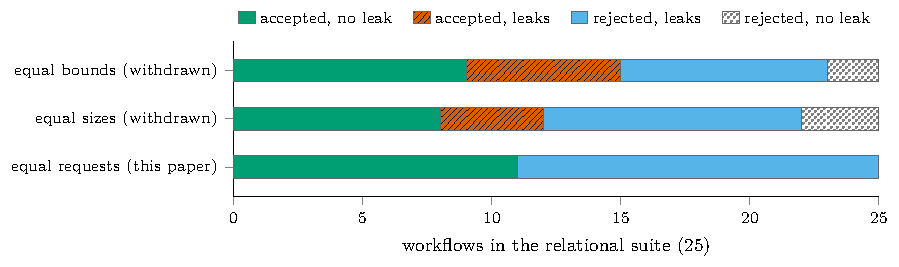
\includegraphics[width=\textwidth]{fig-relational.pdf}
\caption{Verdicts of the three relational rules on the 25 workflows of the relational suite,
against what the runtime shows. The two withdrawn rules accept leaking workflows (hatched);
the content rule accepts only the 11 workflows whose observer never distinguishes the secrets,
and each of its 14 rejections has a witness.}
\label{fig:relational}
\end{figure}

The bounds rule accepts 15 workflows, six of which leak, and the size rule accepts
12, four of which leak. The configuration of the harness before this work (uniform
provider, global keying and estimated billing) detects only one of the size rule's
four leaking acceptances, the one in which the model differs between the arms: the
blind spot of \cref{sec:implementation}, measured. With the provider's answers held
fixed, three of the four leaking acceptances already bill differently under real
tokenizers (E6). The fourth, a redeclared prompt, sends requests of equal token
counts under all three tokenizers, so its leak shows only through a provider that
reads content. Finally, the interval-counting bound of Ngo et al.\ gives between 6.0
and 9.4 bits on the 11 workflows that the content rule proves leak-free, where the
certified bound is zero (E7).

\subsection{RQ3: leakage bounds}\label{sec:eval-leakage}

The leakage suite has eight workflows whose branches test one or two secrets, as
flags or as length intervals, with budgets of 0 to 2 bits (\cref{tab:leakage}). For every workflow, the
number of distinct observations produced by any seed and mode never exceeded the
certified number of classes, and it reached that number in every case: the bound is
attained, as \cref{thm:completeness} predicts. The three workflows whose classes
exceed their budget are rejected.

\begin{table}[t]
\centering
\caption{Leakage suite (E7): declared budget, certified classes and bits, and the largest
number of distinct observations of the trace produced by any seed and mode. The last column
is Ngo et al.'s interval bound, in bits, for the same workflow.}
\label{tab:leakage}
\footnotesize
\begin{tabular}{@{}lrrrrrr@{}}
\toprule
Workflow & Verdict & Budget & Classes & Bits & Observed & Interval \\
\midrule
BalancedNoLeak & accept & 0 & 1 & 0 & 1 & 7.67 \\
ChainedEscalation & accept & 1 & 2 & 1 & 2 & 9.89 \\
FourIntervals & accept & 2 & 4 & 2 & 4 & 9.13 \\
OneBitTier & accept & 1 & 2 & 1 & 2 & 8.42 \\
TwoFlagsThreeClasses & accept & 1.6 & 3 & 1.585 & 3 & 7.75 \\
FourIntervalsOneBit & reject & 1 & 4 & 2 & 4 & -- \\
OneBitNoBudget & reject & 0 & 2 & 1 & 2 & -- \\
TwoFlagsBudgetTooSmall & reject & 1.5 & 3 & 1.585 & 3 & -- \\
\bottomrule
\end{tabular}
\end{table}

\subsection{RQ4: real tokenizers and a real model}\label{sec:eval-models}

The tokenizer facts of \cref{sec:what-fails} are E9, and the harness re-checks the
headline examples live. For the provider assumption, \file{bench/provider/measure.py}
runs SmolLM2-135M-Instruct~\cite{allal2025smollm2,smollm2instruct135m} locally, at a
pinned revision, on fifteen pairs of chat requests padded to exactly equal token
counts under the model's own tokenizer and chat template (E10). Under a shared
sampling seed, all fifteen pairs produced outputs of different lengths, with a mean
absolute difference of 34.1 tokens, while identical requests with the same seed gave
identical outputs in all six trials. Output length is a function of content, not
size, which is exactly the freedom \cref{thm:size-blind} gives the provider. The model
is small, and E10 shows that a real model behaves this way, not how often or by how
much a hosted one does.

\subsection{RQ5: real workflows}\label{sec:eval-real}

\paragraph{Corpus and protocol} The candidates are every workflow defined by the
agent-pattern notebooks of the Anthropic cookbook (7)~\cite{claudecookbooks}, every
LangGraph tutorial notebook (25)~\cite{langgraphrepo}, and the first five user tasks of
each suite of AgentDojo~v1 (20)~\cite{debenedetti2024agentdojo,agentdojorepo}, each
source pinned to a commit. The protocol, the candidate list, the split and every label
were committed before any port was written. Labels are properties of the source,
derived by fixed rules: content from outside the workflow's trust boundary is
untrusted, and for AgentDojo a tool response is untrusted exactly when AgentDojo's own
canary injections reach it; a secret is data that the source itself treats as
confidential. The expected diagnostics follow from the labels: \code{E233} when
untrusted content reaches an effect's argument, \code{E235} when it decides whether an
effect runs, and \code{W237} for a branch guarded by untrusted data whose arms have
different costs. A candidate belongs to the development split if the first
hexadecimal digit of the SHA-256 of its identifier is between 0 and 4 (15 candidates),
and to the held-out split otherwise (37). We wrote the development ports first, then
froze the compiler and checked the 22 held-out ports once against it. The harness fails
if the compiler changed after the freeze without a declared reason, if a candidate is
in the wrong split, if a labelled diagnostic is missing, or if a stretch of prompt text
of at least 20 characters does not occur in the pinned source.

\paragraph{Expressiveness} We ported 30 candidates and excluded 22, each with a
category fixed in advance: the model chooses which node, tool or agent runs next (9);
interactive input, concurrency or timing (4); duplicates that differ only in the model
backend (4); cyclic graphs with more than one back edge (2); reads whose number the
model chooses (1); iteration over a data-dependent count (1); multimodal input (1).
All 20 AgentDojo tasks were ported, as their ground-truth plans executed as fixed
workflows, which is the plan-then-execute pattern~\cite{beurerkellner2025design}
rather than AgentDojo's tool-calling agent. Four of the seven cookbook workflows and
six of the 25 LangGraph tutorials were ported (\cref{tab:corpus}). Seven ports needed
an adaptation that the language forces, such as passing a whole response where the
source extracts one field, or dropping an early exit decided by a response; each is
recorded with whether the certified bound still bounds the source. Five
self-correction loops had to be unrolled, because a \code{retry} body cannot see its
earlier attempts. Porting also forced one change to the language during the
development split: templates could not contain literal braces, so no JSON schema could
be written verbatim, and \code{\{\{} and \code{\}\}} were added as escapes.

\begin{table}[t]
\centering
\caption{The real-workflow corpus by source (E11). ``Held-out'' counts ported
workflows in the held-out split, ``Errors'' ports labelled with an error, and ``Guarantee''
ports whose guaranteed input bound is defined.}
\label{tab:corpus}
\footnotesize\setlength{\tabcolsep}{4pt}
\begin{tabular}{@{}lrrrrrr@{}}
\toprule
Source & Candidates & Ported & Held-out & Errors & Endorsements & Guarantee \\
\midrule
Anthropic cookbook & 7 & 4 & 2 & 0 & 0 & 0 \\
LangGraph tutorials & 25 & 6 & 4 & 2 & 12 & 4 \\
AgentDojo v1 & 20 & 20 & 16 & 13 & 16 & 20 \\
\midrule
Total & 52 & 30 & 22 & 15 & 28 & 24 \\
\bottomrule
\end{tabular}
\end{table}

\paragraph{Agreement with the labels} Fifteen ports are labelled with an error and
fifteen without. Every labelled error was reported, every port labelled clean was
accepted, and the one warning expected on an accepted port (\code{W237} on a routing
workflow of the cookbook) was reported. Two held-out ports received an \code{E233}
beyond their labelled \code{E235}. In both, a value computed only from trusted data,
inside an arm whose guard is untrusted, inherits the guard's integrity: the program
counter imprecision that \cref{sec:labels} removes for confidentiality but keeps for
integrity. These are false positives against the label rule. We changed the harness
after the freeze so that it reports extra diagnostics as imprecision instead of failing
on them; the protocol records this deviation and the two others made after the freeze,
with what prompted each. The 15 rejected ports are accepted after 28 endorsements in
total, one or two per AgentDojo task, four for a corrective retrieval workflow and
eight for a code-generation assistant. Each endorsement marks a place where the source
lets untrusted content decide an effect.

\paragraph{The AgentDojo cross-check} AgentDojo publishes the runs of its attacks. On the
20 ported tasks, its \code{important\_instructions} attack succeeded against
\code{gpt-4o-2024-05-13} 88 times. Every one of the 88 made a tool call that the task's
plan does not contain, or more calls to a planned effect than the plan makes; none
stayed within the plan. The harness fails on a within-plan success against a task the
checker accepts, and there was none. It is therefore the fixed plan, not the checker,
that excludes every recorded attack. The checker contributes something else: in 13 of
the 20 tasks it marks where untrusted content can still steer a planned effect's
arguments or decide whether it runs. In the bill-payment task, for example, the amount
and recipient of the payment come from a file that an attacker can write. The recorded
attacks did not target those places.

\paragraph{Bounds} All 30 accepted variants are certified. The guaranteed input bound is
defined for 24 and undefined for the six that call a model whose tokenizer is not
published, matching the label in all 30 cases. Each port ran 200 times under the
content-dependent provider and the content-sensitive tokenizer, half of the runs with
every text input at its declared byte bound; in the 6,000 runs neither the output
bound nor the guaranteed input bound was exceeded. Re-billing every run's requests with
the port's real tokenizer never exceeded the guaranteed bound either, and the largest
real bill was 0.24 of it. \Cref{fig:real} shows how loose the guarantee is: 4.0 times the
estimate on every AgentDojo port, whose requests carry only inputs, and 19 to 128 times
on the four LangGraph ports with a guarantee, whose later requests carry earlier
responses and pay $\lambda$ bytes per response token. The estimate is not a bound: the
content-sensitive tokenizer exceeded it in 28--100\% of each port's runs, and the real
tokenizers in none of the AgentDojo runs and in 3.5--41\% of the runs of those four
LangGraph ports. Because the runtime writes inputs and responses from a fixed word list
that includes non-English and invented words, these rates describe the mock text, not
a deployment.

\begin{figure}[t]
\centering
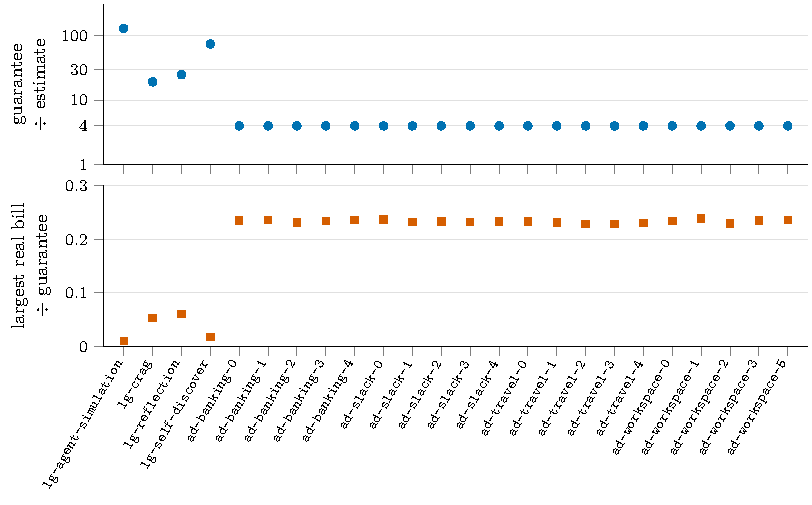
\includegraphics[width=\textwidth]{fig-real.pdf}
\caption{The 24 real ports with a guaranteed input bound. Top: the guaranteed bound
divided by the estimate (log scale); it is 4.0 for every AgentDojo port and 19 to 128 for the
LangGraph ports whose later calls receive earlier responses. Bottom: the largest real-tokenizer
bill in 200 runs divided by the guaranteed bound; no run came within a factor of four of it.}
\label{fig:real}
\end{figure}

\paragraph{The relational analysis} No candidate has a secret, so no port declares one;
\code{E236} and \code{W238} never fired, and every certificate reports a leakage of zero
bits, as it must for a workflow without secrets. On real workflows the relational analysis has, so far, verified
nothing.

\subsection{Analysis cost}\label{sec:eval-cost}

Certifying the 47 synthetic workflows that the harness times takes 0.11\,s in total,
2.4\,ms per workflow, and the 30 real ports, of 17 to 84 lines, take 0.07\,s, the
slowest 3.0\,ms. Both figures include process start-up. The one super-linear step of
the analysis is resolution: the feasible outcome vectors are a product over
independent secrets, each secret contributing a number of vectors linear in its
distinct length thresholds, so their count is exponential in the number of secrets
that guard branches. The implementation enumerates at most 4,096 vectors. Beyond that
it treats every vector as its own class, which keeps \cref{thm:leakage} sound but rejects
a workflow unless its budget covers the logarithm of the vector count. No workflow came
near the limit: the largest number of feasible outcome vectors in any certificate the
harness produces is four.

\subsection{Threats to validity}\label{sec:threats}

\paragraph{Internal validity} The runtime is a mock. Its content-dependent provider is
a hash, which is adversarial in the sense that matters, since any change to a request
changes the answer, but it is not a model; E10 supplies one real model, and a small one.
Re-billing with real tokenizers (E6, E11) applies real tokenizers to the runtime's
requests, whose variable parts are mock text. Relational verdicts are checked by
enumerating declared secret values, which is exhaustive for the suites' small bounds
and would not be for large ones.

\paragraph{Construct validity} The synthetic suites are ours. Their paired design, in
which each unsafe workflow has a safe twin that differs by one edit, stops a checker
from scoring well by rejecting everything, but it does not remove designer bias; the
real-workflow corpus addresses that, but it contains no secrets. The contracts and
$\lambda$ rest on measurement and a structural argument, not on proof, and a tokenizer
revision that changes normalisation could break a contract; for that reason contracts
are tied to revisions and regenerated from measurements.

\paragraph{External validity} The real-workflow corpus draws on three sources and 52
candidates chosen by a fixed rule; it is not a random sample of deployed workflows.
Its labels were derived by rules that we applied ourselves, except that the untrusted
labels of AgentDojo come from AgentDojo's own canary mechanism and the cross-check uses
its recorded runs. The AgentDojo ports are the tasks' ground-truth plans, so neither their
bounds nor the cross-check describe AgentDojo's tool-calling agent. Declared byte bounds
on inputs (8\,KiB where a source gives none) are assumptions that a deployment would
have to enforce. Every assumption the guaranteed bound makes about a provider, its caps
and its envelope overhead, is taken from documentation or framework defaults; no hosted
provider was tested. Finally, the harness's treatment of extra diagnostics was changed
after the held-out results were seen. The change and its cause are recorded, and it
affects only whether the two false positives fail the run, not whether they are
reported.
